\scanpage{73}
\mspage{32}
% Two dark points after 14 are diagonally offset; their punctuation role remains uncertain.
14\unsure{:|..} \uline{Description heuristique des} $\Sigma_i\ \Sigma_{ij}$.
(Peut se préciser considérablement \unsure{dans|ds} un contexte de topologie modérée).
Pour construire $\Sigma_i$, on prend un voisinage tubulaire
\inserted{``standart'' $T_{<i}$} \unsure{\deleted{fermé}|fermé} de
% The insertion leader curves down before the crowded word; both its reading and strike state remain uncertain.
% The dotted left member has Sigma-like top/bottom bars and X-like crossing diagonals. Their temporal order is not established.
$\unsure{\dot X_i|\dot\Sigma_i}=\displaystyle\bigcup_{k<i}X_i$, et on prend
\[
(42)\qquad\Sigma_i=X_i\setminus X_i\cap\mathring T_{<i}
\]
\[
\mathring T_{<i}\overset{\mathrm{déf}}{=}T_{<i}\setminus\dot T_{<i}.
\]
% Oblique note in the left margin, alongside (42) and the following definition.
\margin{\uline{NB} On peut prendre $T_{<i}=\bigcup_{k<i}T_k$,
où $T_k$ est un vois. tub. standart des $X_k$}
(\uline{NB} Il aurait suffit ici de prendre le voisinage tubulaire
standart dans $X_i$ lui $=$, et de prendre donc
$\Sigma_i=X_i\setminus\mathring T_{<i}$)

Pour construire $\Sigma_{ij}$, on prend un voisinage tubulaire
$T'_{ij}$ de $\Sigma_i$ dans
$X_j\setminus\unsure{X_j}\cap\mathring T_{\unsure{<i0|<i}}=X'_i$
% The second X is overdrawn. After the dotted i a separate small closed oval stands a little above its lower hook; its role/degree is not settled.
(NB cette fois-ci il faut \deleted{\unsure{prendre}} d'abord prendre
$T_{<i}$ vois. tub. standart \uline{\unsure{dans|ds}} $X$, ou sinon, dans $X_j$).
On prend $T'_{ij}$ ``suffisamment petit'' p.r. au choix de $T_{<i}$.
Puis on prend $\dot T'_{ij}$\unsure{\deleted{s}|s}, et dans $\dot T'_{ij}$
% The small s-like remnant has a dense lower diagonal; its deletion state is uncertain.
la trace de $\displaystyle\bigcup_{\unsure{i\leq k<j|i<k<j}}X_{jk}$
(donc c'est vide si $j$ est un successeur de $i$), soit $S\dot T'_{ij}$
(``partie singulière'' de $T'_{ij}$.
% No closing parenthesis is visible before the point after this undotted T'_{ij}.

% Left-margin drawing opposite the singular-part paragraph. The middle stroke begins after a visible gap from the filled point.
\figure{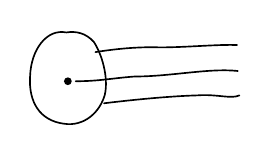
\begin{tikzpicture}[x=.01cm,y=-.01cm,line width=.6pt,line cap=round,line join=round]
\draw (54,11) .. controls (29,6) and (9,33) .. (8,67)
 .. controls (6,99) and (20,123) .. (51,127)
 .. controls (77,131) and (97,112) .. (103,90)
 .. controls (108,68) and (99,38) .. (89,23)
 .. controls (79,12) and (67,9) .. (54,11);
\draw (91,36) .. controls (116,32) and (145,29) .. (173,30)
 .. controls (207,30) and (247,26) .. (271,27);
\draw (66,73) .. controls (96,73) and (113,69) .. (141,67)
 .. controls (187,67) and (236,56) .. (272,60);
\draw (102,101) .. controls (135,97) and (184,92) .. (220,91)
 .. controls (246,89) and (263,96) .. (274,91);
\fill (56,73) circle (1.4pt);
\end{tikzpicture}}

On prend alors un voisinage tubulaire standart
\inserted{$T(S\dot T'_{ij})$} de $S\dot T'_{ij}$ dans $\dot T'_{ij}$,
% One live de stands below the formula's curved insertion leader; no separate cancelled duplicate is isolated.
% The S is reworked; tiny detached dark traces below-left of the following T stem are retained as a local reworking observation, with no invented glyph.
qu'on peut supposer induit par la réunion \inserted{$\bigcup T_k$}
des voisinages tubulaires standart des $X_k$ ($i<k<j$)
dans $\unsure{X\mathbin{\cdot-}X_j|X-X_j}$
% Between the two X groups a detached low dot/short oblique mark precedes one horizontal dash. Its role is uncertain.
(pris ``assez petits'' p.r. aux choix déjà faits de $T_{<i}$
et \inserted{de} $T'_{ij}$).
On \deleted{\unsure{prendra}}\inserted{aura} alors
\[
(43)\qquad\Sigma_{ij}=\dot T'_{ij}\setminus\mathring T(S\dot T'_{ij})
\]
% Pale foliation at the lower left, in another hand; the final display touches the paper edge.
\margin{72}
